% !TEX TS-program = pdflatex
% !TEX encoding = UTF-8 Unicode

% for a word count:
%https://app.uio.no/ifi/texcount/online.php

\documentclass[11pt]{article} % use larger type; default would be 10pt
\usepackage[utf8]{inputenc} % set input encoding (not needed with XeLaTeX)
\usepackage[backend=biber, style=authoryear]{biblatex}
\addbibresource{../bib/software.bib}
\addbibresource{../Literature_Review/Literature/Past_Similar_Work/related_work.bib}
\addbibresource{../Literature_Review/Literature/Network_Analysis/network_lit.bib}
\addbibresource{../Literature_Review/Literature/Bicycling/general_cycling.bib}

%%% PAGE DIMENSIONS
\usepackage{geometry} % to change the page dimensions
\geometry{a4paper} % or letterpaper (US) or a5paper or....
% \geometry{margin=2in} % for example, change the margins to 2 inches all round
% \geometry{landscape} % set up the page for landscape
%   read geometry.pdf for detailed page layout information
%\usepackage{graphicx} % support the \includegraphics command and options
\usepackage[parfill]{parskip} % Activate to begin paragraphs with an empty line rather than an indent
%%% PACKAGES
\usepackage{hyperref}
\usepackage{booktabs} % for much better looking tables
\usepackage{array} % for better arrays (eg matrices) in maths
\usepackage{paralist} % very flexible & customisable lists (eg. enumerate/itemize, etc.)
\usepackage{verbatim} % adds environment for commenting out blocks of text & for better verbatim
%\usepackage{subfig} % make it possible to include more than one captioned figure/table in a single float
\usepackage{graphicx}
\graphicspath{{../images/}}
\usepackage{caption}
\usepackage{subcaption}
\usepackage{multirow} % allows multiple rows per cell
% These packages are all incorporated in the memoir class to one degree or another...

%%% HEADERS & FOOTERS
\usepackage{fancyhdr} % This should be set AFTER setting up the page geometry
\pagestyle{fancy} % options: empty , plain , fancy
\renewcommand{\headrulewidth}{0pt} % customise the layout...
\lhead{}\chead{}\rhead{}
\lfoot{}\cfoot{\thepage}\rfoot{}

%%% SECTION TITLE APPEARANCE
\usepackage{sectsty}
\allsections

{\sffamily\mdseries\upshape} % (See the fntguide.pdf for font help)
% (This matches ConTeXt defaults)

%%% ToC (table of contents) APPEARANCE
\usepackage[nottoc,notlof,notlot]{tocbibind} % Put the bibliography in the ToC
\usepackage[titles,subfigure]{tocloft} % Alter the style of the Table of Contents
\renewcommand{\cftsecfont}{\rmfamily\mdseries\upshape}
\renewcommand{\cftsecpagefont}{\rmfamily\mdseries\upshape} % No bold!

%%% END Article customizations

\title{\vspace{-3.0cm}The Suitability of Open Street Map Data for Defining Urban Bicycle Networks}
\author{Hugh Kelley}
%\date{} % Activate to display a given date or no date (if empty),
         % otherwise the current date is printed 

\begin{document}
\maketitle
\section{Abstract}
\tableofcontents
%\listoffigures
\listoftables

%%%%%%%%%%%%%%%%%%%%%%%%%%%%%%%%%%%%%%%%%%%%%%%%%%%%%%%%%%%%%%%%%%%%%%%%%%%%%%%%%%%%%%%%%%%%%%%%
%%%%%%%%%%%%%%%%%%%%%%%%%%%%%%%%%%%%%%%%%%%%%%%%%%%%%%%%%%%%%%%%%%%%%%%%%%%%%%%%%%%%%%%%%%%%%%%%
\section{Research Goal and Overview}

What makes a city comfortable for cycling? The conditions are clear when one sees them, but defining the characteristics quantitatively is challenging. 

This research intends to define the overall suitability of a city to cycling using estimates of the roads cyclist are and are not willing to use and the effect these decision have on travel times. The central research question is: \textit{how does a peference for safety decrease accessibility in central London when traveling by bicycle?} It extends the literature in three ways; extending quantitative research to a holistic approach rather than focusing on individual edges or nodes, extending holistic approaches to quantitative outcomes rather than visual or anecdotal conclusions, and by emphasizing the use of open source tools and data that are available to any member of community. 

The research provides a methodology that allows a community to identify nodes and edges for improvement that will have the largest impact on the overall network, quantify the expected improvement, and thus require from elected officials specific changes to the roads in their communities. 

The subquestions addressed in the methodology are, What is the quality of the Open Street Map metadata for streets in London? How important are the OSM highway types to efficient transit within London? How does transit by bicycle compare to transit by public transport within London? 

The issue implied by these research questions is: to what extent is street level transportatoin space a zero sum game? Can a high level of service for cyclists be built without taking large amounts of important space away from automobile trafic? 

The intended outcomes of this research include(1) an understanding of the roles of location and connectivity for cycling infrastructure and (2) an understanding of the usefulness of Open Street Map data for estimating these sorts of measures. 


\subsection{ethical risks}

This project relies entirely on publicly accessible data. For this reason, ethical risks are not present in the research methodology.  

%%%%%%%%%%%%%%%%%%%%%%%%%%%%%%%%%%%%%%%%%%%%%%%%%%%%%%%%%%%%%%%%%%%%%%%%%%%%%%%%%%%%%%%%%%%%%%%%%%%%%%%%%%%%%%%%%
\section{Introduction}

Cycling in cities generally

Cycling in London

safety

need for open data and methods for people to advocate in places where local government is not supportive

More than half of the world's population lives in cities. Cycling is of obvious importance to the well being of the world's  urban population in terms of the macro-climate crisis, local pollution problems,  public health, wealth disparaities, and urban traffic congestion. A commonly researched question is ``what factors have the most significant effect on cycling rates?'' The research has only recently begun to address cycling from a network perspective. 

A large body of research addresses the factors influencing the decision to cycle in an urban environment, and which factors make cycling in that environment more or less safe. Modern quantitative methods have only begun to be applied to this problem though. Challenges come through the lack of technical knowledge among interested parties, lack of access to tools for analysis of this type of complex spatial problems, and lack of access to the data necessary to define the nature of the problem and estimate the outcomes of possible solutions. 

 The review of literature that follows will argue that the majority of work on this question approaches the matter from a perspective of discrete policy intervention and the effect of marginal improvements on cycling. This fails to build a comprehensive theory of cycling rates that a network analysis approach can offer. Only network theory can offer a high level look at the level of service in a community. 

Thus a comprehensive approach to encouraging cycling in an urban area would consider individual improvements in the context of the existing network, and how the improvements would change the size of the low-stress nework coverage of the city. 

This literature review will show that existing research is limited by two considerations. First is the scope of the analysis, considering individual changes instead of the status of the entire transportation network from the cyclists perspective.  Second is the difficulty of obtaining data used by the studies that do take a comprehensive network approach. 

After critically reviewing this existing research, a methodology for using open source tools and data to estimate the relative strength of a cycle network and a method for prioritizing improvements will be specified. 

The review that follows takes the structure of an initial look at typical literature considering how to promote cycling, recent attempts to use network analysis to accomplish this same goal, and closes with a look at work in network analysis that can inform applying the field to cycle networks.

 The implication of this view is that infrastructure changes are unlikely to have a meaningful effect on behavior in the system until a critical mass or tipping point is reached in the network. 

Basic attitude is that improvements to infrastructure only matter to the extent that they improve safe connectivity to ``important'' nodes/edges. 

In this context, this work hopes to make a contribution using London as a case study. London is an attractive case because it has a considerable cycling population but does not yet have the level of infrastructure that exists in world leading cities like Copenhagen. Thus London's position at a mid point of cycling infrastructure development allows strengths and weaknesses to a live program of improvement to be identified. 

\subsection{Research Structure}

First, existing work on this research area will be reviewed and the techniques to be built upon will be identified.  Then a methodology for defining the strength of cycling infrastructure in a city will be specified. The data available for analysis will be described in the context of past work, and what is available for other cities and through other channels that were not available to this research. the steps taken for data cleaning, transformation and joining will be specified. Section 3 will describe the implementation of this methodology for London, identifying the scope of the case study, defining the exact data collected and transformed and the specific tools used. 

The multiple stages of results will be reported, and interpreted. Finally conclusions will be drawn, areas of further research specified, opportunities to improve the methodology and the quality of the data emphasized and the key recommendations for further improving the London cycling infrastructure network will be made. 


\subsection{The role of the researcher}

Read other versions of this and see if it makes sense for this 

%%%%%%%%%%%%%%%%%%%%%%%%%%%%%%%%%%%%%%%%%%%%%%%%%%%%%%%%%%%%%%%%%%%%%%%%%%%%%%%%%%%%%%%%%%%%%%%%%%%%%%%%%%%%%%%%%

\section{Literature Review}

\subsection{Cycling Behavior Research}

The most important conclusions from literature that tries to predict cycling behavior is the focus on multiple types of cyclists, and the factors that influence each type's decision to cycle. Most often, four types of cyclists are used, ``strong and fearless'', ``enthused and confident'', ``interested but concerned'', and ``no way no how'' (\cite{dill2013four}). This categorization is sometimes changed to follow demographics, focusing on young, generally male, adults, older adults, and childern. CITE. The literature separates the decision to cycle into the decision of cycling frequency, how often someone who is willing to cycle generally chooses to do so, and the decision to cycle at all, with different factors influencing each decision (\cite{stinson2005comparison}). 

Despite behaviorial differences between these categories, research has shown that all cyclists are willing to sacrifice time and energy for increased safety on their route. CITE. Indeed, psychological research showed that fear is a significant factor during an urban cycling trip (\cite{ellett2018state}). This is important given the sensitivity cyclists show to efficiency. CITE. The impact of a route change can be very significant, for instance a higher frequency of stop signs on a route can double the energy required for a journey (\cite{fajans2001bicyclists}). Given the common trade off between efficiency and safety, it was found that the effect of infrastructure improvements is very dependent on context, effect is a function of the change in safety, and the importance of the location to trips (\cite{kondo2018bike}), improvements that meaningfully increase safety at important locations have the largest effect. 

Several studies looked at the importance of perception in behavior change, assuming that a real change in safety is irrelevant if it is not perceived by potential cyclists as a change(\cite{li2012physical} and \cite{parkin2007models}). This gives rise to literature that focuses on a behavior and attitude change approach from psychology the prioritizes change in habits and perception over infrastructure, with changes to the built environment only used where required to change perception (\cite{savan2017integrated}). This should be considered in the context of research showing that cyclist perceptions of danger are generally accurate (\cite{vandenbulcke2014predicting}). Thus it seems reasonable to conclude that despite the decision to cycle being a fairly complex mix of factors, the decision for almost any urban commuter, comes down to safety, and efficiency. An efficient network of safe edges, connecting important nodes, would be expected to have a meaningful effect on the rate of cycling in an urban area.  


\subsection{Literature addressing cycling From a network perspective}

\cite{buehler2016bikeway} is a very useful introduction to the literature on cycling networks. Unfortunately it concludes that very little true network analysis has been developed for cycle networks. The majority of papers they found could be categorized into those that focus exclusively on nodes, and those that focus on edges of the dual graph, where intersections are nodes and streets are edges. At the time of writing there were 115 papers citing Buehler's review, however all but 5 of them fail to take Buehler's central recommendation that \textit{If individual characteristics of a network's links and nodes contribute to cycling levels, it logically follows that a network of such features would as well...}. The ``Toward Studying the Whole Bicycling Network'' section of Buehler's review is a good overview of attempts up to 2016. The key findings were that continuity and connectivity of infrastructure is valued by cyclists. Of particular interest is the \cite{schoner2014missing} study of the relationship between network characteristics and cycling mode share in 74 US cities. That study found density of the network had the highest elasticity for effect on cycling rate. 

Several of the works reviewed contribute new ways of measuring ``quality'' of the infrastructure, these quality measures include a Bicycle Compatibility Index (BCI) (\cite{klobucar2007network}),  Bicycle Level of Service (BLOS) (\cite{lowry2012assessment}), and Level of Traffic Stress (LTS) (\cite{mekuria2012low}). Each of these can reasonably be viewed as an attempt to measure the ``safety'' of a network link. These studies generally lacked a rigorous method for prioritizing nodes by importance or defining a sample set of trips between nodes. Improvements to this will be addressed in the section reviewing network analysis literature. 

Buehler notes that a key challenge to using the network methods reviewed is data availability, this research hopes that network analysis can be a method for reducing rather than extending the amount of data necessary to understand a cycle network, as network statistics could be used to replace some empirical measurements as discussed below.  They further criticize the approaches as lacking empirical validation. Gathering accurate cycle traffic data and safety data is an immense challenge as demonstrated by the flow estimation techniques of \cite{gosse2014estimating} and the safety estimate techniques of \cite{puchades2018role}, which focuses on near misses as a proxy for predicting actual safety incidents, but acknowledges the difficulty of collecting near miss data without human observation. CITE. 

Since the publication of Buehler's review, the papers extending the full network analysis method have had moderate success. \cite{akbarzadeh2018designing} uses taxi trip data to weight the links between destinations in order to build communities of nodes that tend to be origin and destination pairs. While this is a novel approach to prioritizing edges, taxi usage tends to be for less frequent travel between nodes and the general literature as well as this work focuses on daily commuting, which is rarely accomplished by taxi. \cite{boisjoly2019bicycle} focuses on the directness of routes on cycle paths between nodes. 

\cite{doorley2019designing} focus on building cycle infrastructure to maximize a function of travel costs, infrastructure costs, health, traffic accidents, and pollution. While this is an interesting approach, it addresses a more political question in the sense that the key result of the algorithm is to recommend a specific amount of investment in cycle infrastructure to maximize the costs and benefits to all road users, The author's fail to recognize the prioritizing the goals of public policy is a highly normative and subjective exercise and that a model designed to give an ``objective'' answer to this question inherently reflects the author's preferences and when calibrated to ``the real world'' reflects the biases and preferences of the status quo, rather than the true ideal outcomes preferred by a population. Instead, modeling, especially for urban planning purposes, should accept an exogenous goal and implement it as efficiently as possible. For instance, cycle infrastructure, is explicitly intended to reduce motor vehicle use, it would make no sense to then use a model that determines the efficient level of motor vehicle use, the political process has already determined the answer and merely asks for implementation recommendations from the modeler. 

\cite{mauttone2017bicycle} similarly focuses on an optimization framework for cycling networks, choosing a subset of streets that are ``suitable to building cycle infrastructure''. This is odd in the sense that the goal of building cycle infrastructure is to \textit{create} streets that are suitable for cycling, not merely identify them. Similar to \cite{doorley2019designing}, they identify a cost to building cycle paths which they seek to balance against the benefits. 

Overall, it is not clear that a model for building cycle paths should be particularly cost sensitive. \cite{gu2017cost} found a very high return on investment to the budget for cycling infrastructure in New York City. The very idea of using network analysis for the development of cycle networks emphasizes the potential non linearity of the effect of building more infrastructure, with usage accelerating as the network approaches ``completeness'' in some for. In addition, cities tend to combine cycle infrastructure improvement with other required improvement and maintenance activities, mitigating the costs by being opportunistic in implementation. 

Lastly, \cite{osama2017models} uses a number of predictors including network statistics to predict bike travel within zones of Vancouver similar to \cite{schoner2014missing}. They found a positive coefficient for the density of the bike network in the zone. 

Thus while network analysis has been applied to cycle infrastructure, clearly there is not a consensus on the methodology. In particular, a definition of ``quality'' or ``safety'' has not been established. Additionally, a method for exploring the network of infrastructure defined is still lacking. Lastly,  

\subsection{Research on the quality fo Open Street Map Data}

%%%%%%%%%%%%%%%%%%%%%%%%%%%%%%%%%%%%%%%%%%%%%%%%%%%%%%%%%%%%%%%%%%%%%%%%%%%%%%%%%%%%%%%%%%%%%%%%%%%%%%%%%%%%%%%%%%


\subsection{Network analysis Literature relevant to the research methodology proposed}

\textit{note: this section should probably be worked into the review of cycle network analysis above instead of separated out. Combine criticisms of existing work and solutions from network science.}

This work intends to improve upon the work detailed above through the inclusion of more ideas from network science that can improve and extend and simplify the models already specified. 

There are a number of considerations from network analysis literature that can complement the work already applying the field to cycling networks. Perhaps the most important is the idea that the transportation network and the location of activities in a city reinforce each other. The most productive activities that occur in a city tend to be the most easily accessed according to central place theory. This has been shown empirically for instance by \cite{porta2012street} and by \cite{wang2011street}. In the literature discussed above authors address the key change in networks of defining a computationally feasible set of trips between nodes in a few different ways. This is misguided though as network theory offers a number of tools for exploring a graph efficiently. A random walk weighted by a centrality measure will tend toward trips between more important nodes because these tend to be more central. For instance \cite{Jiang2009characterizing} or  \cite{volchenkov2007random} both show that weighted random walks can do a accurate job of representing human activity on a street network. 

A number of network statistics are used in the literature reviewed above. \cite{crucitti2006centrality} complements these as the centrality and connectedness measures used should be more formally justified according to network theory. 

While, the multiplex offers an interesting approach to studying the interaction between bicycle usage and train and bus, this is beyond the scope of this work and perhaps beyond the scope of London , where bicycles are not generally allowed on public transport, unlike some other cities. 

The potential for a ``transition'' in the cycle network per \cite{barthelemy2018transitions} is an exciting possibility. Finding edges that need to be added to a network in order for a transition in network connectivity to occur is a valuable exercise. In addition, specifying network characteristics according to those specified by \cite{barthelemy2011spatial} is also very valuable. 

Overall there are a number of considerations from network science that this research intends to add to the analysis of cycle networks. The exact implementation of these considerations will be specified in the methodology section. 

%%%%%%%%%%%%%%%%%%%%%%%%%%%%%%%%%%%%%%%%%%%%%%%%%%%%%%%%%%%%%%%%%%%%%%%%%%%%%%%%%%%%%%%%%%%%%%%%%%%%%%%%%%%%%%%%%
% Methods and Data need a good structure because they rely on each other
\section{Methods}

%%%%%%%%%%%%%%%%%%%%%%
- define scope, minimize area while capturing the largest number of trips by bicycle, trips in total, road casualties, and households and jobs. This will be some part of central London. 
-- build boundary based on scope using postgis and qgis
- define filters for OSM data
-- this includes trying to understand the relationship between relations and individually tagged edges and nodes. 
-- pictures of network, specific edges, and photos of real life infrastructure. 
-build networks from data
-- removing streets
-- undirected
- identify network nodes closest to lsoa centroids
-compare \% of trips possible across Quant, bike 1, bike 2, and undirected versions. 
- compare change in directness between bike 1 and bike 2.  
-- compare bicycle accessibility to Quant
%%%%%%%%%%%%%%%%%%%5


\section{Most optimistic Project Plan/Methodology}

Goal is to quantify the quality of the London Cycling Network with the working assumption that a better network has a meaningful positive effect on the rate of cycling in a city. 

The first step in this investigation is to build a data set that represents the London cycling network as accurately as possible. This representation needs to reflect the fact that different cyclists are willing to use different streets as a function of the perceived safety of the street and the level of confidence of that cyclist. Thus the data set will be multiple representations of the city cycling network that each represent a level of confidence, only including streets with a certain level of safety. 

A key question then is, how to quantify ``safety''. In a perfect world, this would be done empirically. This would involve a combination of cycle traffic volume collection, cycle traffic behavior observation, and interviews with a representative set of cyclists and non-cyclists about their decision making. All of this data could be compared to the cycling environment in different locations to find cyclist sensitivity to different factors.  

The literature provides a number of methods, which will be explored to the fullest extent possible. Factors that will be considered include, the presence of dedicated bike infrastructure, traffic volumes, traffic speeds, road characteristics, historical traffic incidents, and intersection characteristics. 

Once the network has been quantified in this way, two basic methods will be applied to evaluate it. The first is to compare the distribution of edges by centrality for each of the networks. Are cars and high confidence cyclists at a significant advantage in terms of the edges available to them compared to lower confidence cyclists? Does does the centrality of edges allowed under the most conservative standards explain many Londoner's choice not to cycle at all? 

The second method is intended to extend the first. Looking at the distribution of centrality is unable to reveal the network's actual service for common trips between important nodes on the network, because a high number of very central but disconnected edges is not as useful as a high number of high centrality edges with high connectivity. To investigate this, a random walk between nodes, weighted by node importance will be used. This will build a sample of trips and statistics about the random walk can be used to compare the experience of representative users of different networks. 

Finally, the possibility of a ``transition'' in the networks defined will be explored. What changes to the network are required for a dramatic change in connectivity to occur? This is the most uncertain but potentially most valuable part of the research. Past research has analyzed the linear individual effect of cycling infrastructure, but has not considered the possibility of a rapid acceleration in cycling usage as the result of a network wide transition in connectivity. 

Finally, community identification could be applied to the networks to find whether particular neighborhoods in London are especially good for cyclists. 

 

\subsection{Data Sources}


\section{Data considerations}

I still need to spend a lot of time with OSM, networkx, and the London data store. 
OSM has street network data, bike network data and some road characteristics. 
Networkx should be able to turn this data into a usable file. 
The London data store has traffic incident data but I haven't found data with exact locations yet
There is traffic volume data but it's at a few thousand observation points, so a continuous data set needs to be estimated. 
I think OSM is my only source for street characteristics, not clear that it's accurate or up to date.
Official data for cycle infrastructure is from 2014: \href{https://data.gov.uk/dataset/47f0a282-3356-4530-8e7b-f67aaf4bec63/cycle-routes}{link}
This says it's updated and maybe integrated into OSM? \href{https://www.cyclestreets.net/blog/category/open-data/}{link}
Press release about data set \href{https://www.london.gov.uk/press-releases/mayoral/action-plan-to-get-more-londoners-cycling}{link}
But no actual data. Seems like OSM is the delivery mechanism, unclear how integrated the data is into OSM. 

\subsubsection{Open Street Map}
Open street map provides community generated geospatial data. This data is accessible via the overpass API from several hosts. 
Geoff Boeing describes using th OSM API query language as "notoriously difficult". CITE

\subsubsection{A Close Look at an Open Street Map Case Study}

Open Street Map is a mapping project started in 2004 to collect volunteered geographic information. It consists of geometries drawn by users, either in person, as they travel through a city or remotely, looking at donated satelite images of cities. 

Cite OSM wiki page
https://en.wikipedia.org/wiki/OpenStreetMap

Second to the actual geometry of a "way", streets and paths, node, single point on the map, or relation, collection of ways nodes and other relations are tags. Tags specify what a particular geometry is, what its characteristics are, and rules for use or other characteristics of the geometry. This allows for differentiation on the map between public and private areas, specification of what exactly a node is referencing, an intersection, mailbox, or a business location, or the type of traffic allowed or commonly seen on a street way. 

There are four possible problems with Open Street Map, missing geometries, inaccurate geometries, missing tags and innaccurate tags. The review of literature will provide detail on attempts to measure the accuracy of the data in Open Street Map. 

Using data from Open street map is difficult. 

Compare Relation = cycleway to a list of edges and nodes tagged cycleway

Adding living streets and residential streets don't do much. 

Part of the problem is the lack of consistent tagging, it only takes one line segment missing a tag to disconnect two nodes,

but this also reflects the fact that getting somewhere within London nearly always requires leaving cycle infrastructure at some point and using main roads. 

The importance of this consideration will be shown using a percolation style analysis of the network, adding busier and busier roads to the network and considering the largest connected component. 

%%%%%%%%
% image of OSM London cycle network by relation
% image of OSM London cycle network by tag
% image of OSM missing tag situation from Overpass turbo
% image of same location street view
% image of OSM implied cycle infrastructure
% image of real street without cycle infrastructure. 
%%%%%%%%%%%%%

Two basic problems for using OSM data to define cycling networks were found. The first is that defining the network by relation exagerates the network, the second is that relying on the metadata tags of individual features understates the cycle network. Looking at OSM it is clear that the relations identifying bike routes are not reflecting sets of ways and nodes with a given tag, or reflecting streets and intersections where cycling is meaningfully safer than other streets and intersection. At the same time, it is clear that there are many ways and nodes that are more accomodating to cyclists than their OSM metadata indicates. 

In the case of the relation, Quietway XXX was examined in person. figure XXX shows an image of Brandon rd, a part of the quiet way. this way is tagged
Brandon rd is part of OSM relation XXX the Hackney Camden cycle route.  this road though, as can been seen in the image, has no actual cycle inrastructure. This in Open street map, it is tagged as an unclassified highway. There is a tag noting the max speed is 20 mph. Data collected for 20 mph streets found that as many as 80\% of drivers exceeded these limits. 
https://www.thesun.co.uk/news/7253694/20-mph-zones-cause-more-deaths/

In other cases, osm underestimates the quality of cycling infrastructure. for instance the intersection of Mile end Road and Cambridge Health Road in the borough of tower hamlets is a high traffic intersection both for automobiles and for cyclists. It is an integral part of the Stratford to Aldgate cycle super highway. This intersection has been reworked to be safer for cyclists. In open street map though, it i labeled a "trunk" highway, due to its high traffic nature. It is way 7058092014. There is also a tag cycleway:left=lane indicating that there is a cyclelane on the left side of the street. 


\subsubsection{2011 Census Journey to work data}

The 2011 census asked questions about where people work and how they get there. 

This data is shared through the Nomis Labor Force website as multi-sheet excel pivot tables. Making the data usable required, stripping the meta data headings from each sheet, importing the book to pandas dataframe by sheet, melting from a picot table to long data with origin, destination, and count columns, adding the sheet name that identified the mode of travel as a column, appending each individual sheet together into a single dataframe, and pushing the dataframe to the sql database. 

Exact specifications for pulling data out of Nomis service

\subsubsection{LSOA boundaries and data}

where LSOA's were comprised of multiple polygons, the centroid of the largest polygon was used. 

lsoa population from mid 2011 

https://www.ons.gov.uk/peoplepopulationandcommunity/populationandmigration/populationestimates/datasets/lowersuperoutputareamidyearpopulationestimates

LSOA boundaries are available from the London Data store



https://data.london.gov.uk/dataset/statistical-gis-boundary-files-london

On maps created using these boundaries the copyright must be stated. This is
%"Contains National Statistics data © Crown copyright and database right [2015]" and "Contains Ordnance Survey data © Crown copyright and database right [2015]"

\subsubsection{Road KSI data}

https://www.gov.uk/government/collections/road-accidents-and-safety-statistics

https://data.london.gov.uk/dataset/pedal-cyclist-casualties-killed-and-seriously-injured

https://data.london.gov.uk/dataset/road-casualties-severity-borough

Factors preventing a closer understanding of road stress/danger. 
	Lack of traffic flow data
	lack of road network quality over time
	difficulty of defining actor behavior around time of crash
	difficulty of associating incident with edge.  

\subsection{Data import, storage, cleaning, and joining}

data import was done in python using the csv, pandas, geopandas, json, and osmnx packages. Once the data was cleaned, it was passed to a postgres database with the postgis extension using the sqlalchemy package. Postgis was used for calculating distances, associating nodes with centroids

remove multipolygon lsoa interior rings in favor of polygon lsoa shapes

\subsection{Defining Cycle Networks}

How were the representative networks built? 

Open Street Map uses tags to associate street characteristics with the geometries that make up the map. Appendix XXXX contains the definitions from the OSM wiki page for each of the tags used. Most important to note is that this research uses 5 ``levels'' of street stress. The highest level allows all street conditions. The second level allows all but ``primary'' streets, the largest busiest streets. Then ``secondary'' streets are removed in the third filter. ``Tertiary'' type streets are moved to build the fourth filter. The fifth filter moves ``living streets'' and ``residential'' streets which both are specified to be low traffic streets used primarily for local trips. Thus the most conservative layer of the network contains only edges where there is no expectation of interaction with motor vehicles. 

The networks were simplified so that a node with degree 2 was removed and the two edges were joined, becoming a continuous path way. 

\subsection{Travel Times}

Travel times can be calculated using the networkx package CITE. 

\subsection{Accessibility}

\subsection{assumptions and concerns}

used centroids instead of actual nodes from Quant Data


%%%%%%%%%%%%%%%%%%%%%%%%%%%%%%%%%%%%%%%%%%%%%%%%%%%%%%%%%%%%%%%%%%%%%%%%%%%%%%%%%%%%%%%%%%%%%%%%%%%%%%%%%%%%%%%%%
\section{Analysis \& Results}

\subsection{Defining Scope}

Goal is to capture the largest computationally feasible network with a simple set of rules. 

The first rule was to restrict the network to ``inner london''. This has the advantage of a formal designation by the GLA for each borough, capturing, XXX\% of the population with a population density of XXXXXX compared to XXXXX for london overall, XXXXXX\% of the jobs in the city, and XXXX\% of the journey's to work. Additionally, rates of cycling are higher in inner London than in the periphery. 

Second, the area of interest was restricted to north of the river Thames. This captures XXX\% of the population, with a density of XXXXXXX, XXX\% of London's jobs, and XXX\% of the journey's to work. Further, it has the advantage of excluding the need to cross the river, where journey's are focused on a few number of bridges, with a significant effect on the shortest paths, reducing the effect of other changes on the network. 


Each network is created using a filter that excludes Open Street Map features tagged with certain values. All features tagged with ``bicycle=no'' or ``service=private'' were excluded. Additionally, where the edge's ``highway'' tag was ``footway, steps, corridor, elevator, escalator, motor, proposed, construction, abandoned, platform, or raceway the feature was also excluded. 

The most aggressive bike filter used only these conditions.


%%%%%%%%%%%
% This needs more work for justification
%%%%%%%%%%%%%%%



 

\subsection{Defining Networks}

Five network definitions were considered. The exact filters used to select this data are available in APPENDIX XXXX 

The first network is the set of edges where a cyclist can expect to travel without interacting with motorized traffic at all. This is separated cycle routes, tow paths, and other segregated ways. 

The second builds on the first by adding ways tagged as living streets and residential streets.

The third adds all public streets where cycling is not forbidden. 

The fourth network is an undirected version of the third network. This is used to consider the effect of one way restrictions on travel times. 

The fifth network is made up of the cycleways designated by TfL on Open Street Map. This is an interesting case because a significant part of this network is made of routes without cycle infrastructure. The network is considered in the sense that, if this was to become a high quality, low stress network, how well would it serve journeys in London? 

Building networks using Overpass API queries proved to be a tremendous challenge. There are two possible approaches to building an Overpass query filter, positive and negative filters. OSMnx relies on negative filters, including everthing but what is specifically excluded. This was the type of filter used for the 5 levels of networks studied, with more conditions added to take out additional highway types. The trouble that arises with a negative filter though is that an edge that is tagged, highway = primary, and tagged separately with a cycle related tag will be excluded. This was a problem for instance where cycle infrastructure was tagged, not as a separate edge, but as metadata using for instance "cycleway:left=lane" key value pair. the negative filter removes the edge because it has the "highway=primary" tag and a method for including based on the cycle tag was not found. Likewise, the "bicycle" key could have several values including no, designated, and permissive

Further, OSMnx retrieves ways with a highway tag as in way[highway=cycleway]

This ruled out using the filter relation[route=bicycle]  which would collected all nodes and ways included in any relation tagged with route-bicycle. 

Thus the networks built using a  full combination of conditions were not possible. 

good example of the difficulty of building a good network representation is castle baynard st. It connects the central london part of cycle superhighway 3 with the east london section that continues out to limehouse. this is a tunnel that serves as a bike path and as a driveway of sorts to an underground car park. 

insert picture of castle baynard street. A network built from the relation[route=bicycle] set of ways and nodes would include this but the negative filters do not. 


\begin{figure}
\centering
\begin{subfigure}{.5\textwidth}
  \centering
  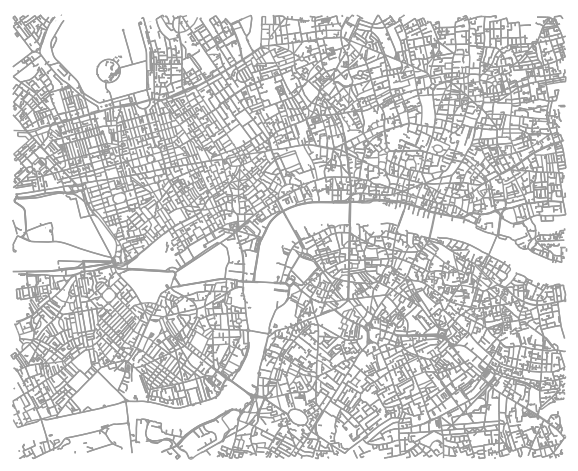
\includegraphics[width=1\linewidth]{bbox_bike_1_filter_cropped}
  \caption{1: most confident cyclists}
  \label{fig:sub1}
\end{subfigure}
\begin{subfigure}{.5\textwidth}
  \centering
  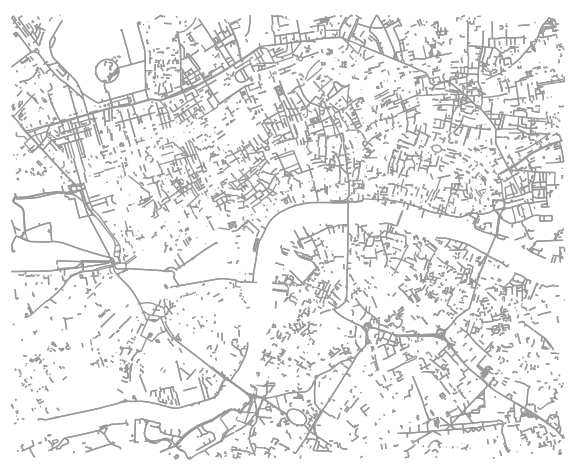
\includegraphics[width=1\linewidth]{bbox_bike_5_filter_cropped}
  \caption{5: no interaction with cars }
  \label{fig:sub2}
\end{subfigure}
\caption{Edges included by different filters}
\label{fig:test}
\end{figure}

\begin{figure}
\centering
\begin{subfigure}{.5\textwidth}
  \centering
  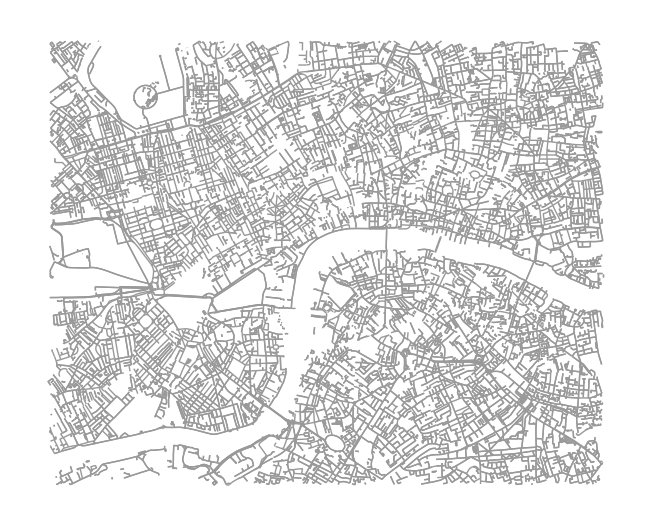
\includegraphics[width=1\linewidth]{bbox_bike_2_filter_cropped}
  \caption{2: all but primary streets}
  \label{fig:sub1}
\end{subfigure}
\begin{subfigure}{.5\textwidth}
  \centering
  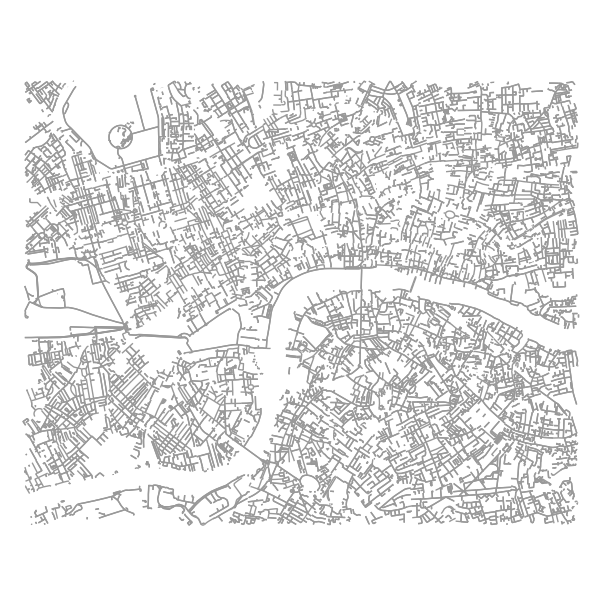
\includegraphics[width=1\linewidth]{bbox_bike_4_filter_cropped}
  \caption{4: only residential and living streets}
  \label{fig:sub2}
\end{subfigure}
\caption{Edges included by different filters}
\label{fig:test}
\end{figure}


%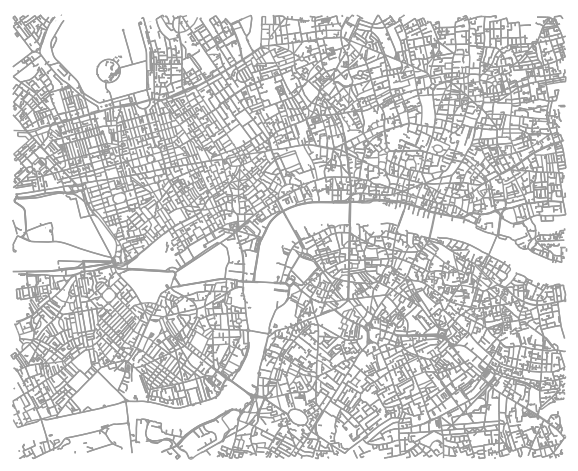
\includegraphics{bbox_bike_1_filter_cropped}

%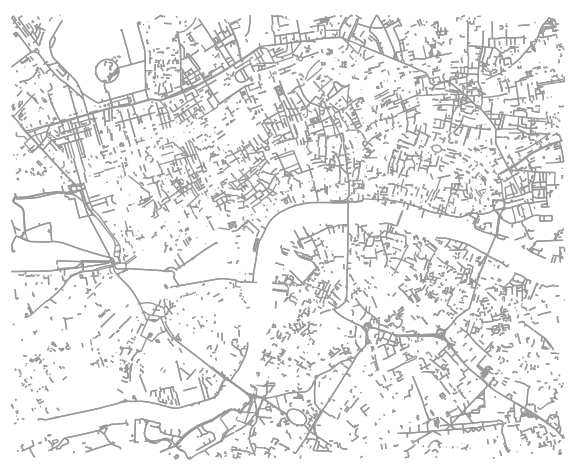
\includegraphics{bbox_bike_5_filter_cropped}
Level\_1

all streets using the OSMnx bike filter

Level\_2

level\_3

Removes trunk, primary, and secondary streets. 
the size of the network here is pretty substantial but connectivity is still bad. 

Level\_4

excludes all streets except for living streets and residential streets

there are XXXXXXX separate networks here with an average of XXXXXX edges each

level\_5

excludes any edge where a cyclist might interact with motorized traffic. this is barely a network, it's just a collection of infrastructure features. 


Undirected 1

This is level\_1 but with the street directionalities removed

Undirected 2

This is level\_2 but with the street directionalities removed





Level\_5


no interaction with cars

because this was a negative filter many nodes were excluded needlessly. 

check this, why isn't the regents bike path fully included?


\subsection{Network Characteristics}

chart of largest connected component of network as edge types are included. 

no cars,
+ living streets
+ residential streets
+ tertiary 
+ secondary
+primary

\subsection{Travel Times}

As seen table XXXXX travel times for bike network 2, without trunk or primary highways, are substantially longer than travel times for bike network 1. This indicates that the effect of removing these edges is not just to disconnect the network but also requires a network user to take a less direct route, straying further from the straight line between origin and destination. 

The difference between directed and undirected distances is also notable. 

the standard deviation 

the min is unchanged, while the max 

Travel times by bicycle for aggressive cyclists are XXXXX compared to the QUANT travel times by public transport. 

\subsection{test for differences}

There's got to be a significant difference between the distances for the different networks right?

\subsection{changes in routes}

Seen in figure XXXX  compare longest path for directed network 2 to the path between those nodes in directed network 1. 

Compare longest path for directed network 1 to undirected network 1. 

compare o/d pair with largest increase in distance between directed 1 and directed 2 to the distance in undirected 2. 

Is allowing travel in any direction on side roads a good replacement for primary and trunk routes?

\subsection{Accessibility} 

in qgis, color lsoa's by travel time to central lsoa. 

in QGIS color lsoa's by travel time from lsoa with highest average distance. 

in QGIS color lsoa's by  average directness, distance divided by straightline distance. 

Plot a few paths in osmnx to look at low directness. 

\subsection{Notes about computation}

runtimes for the distances between nodes were long. computations were done on an intel i74700HQ processor with the database contained on the internal Solid State Drive. 

Runtimes increased with the number of connected origin destination pairs, since unconnected pairs  did not require the calculation of a shortest path. Thus bike 1 travel times took longer than bike level 2. Additionally, the undirected network calculations took substantially longer than the directed networks because there were sugnificantly more route possibilities with more edges available at each node. 

Tale XXXX contains calculation times by network type. 




%%%%%%%%%%%%%%%%%%%%%%%%%%%%%%%%%%%%%%%%%%%%%%%%%%%%%%%%%%%%%%%%%%%%%%%%%%%%%%%%%%%%%%%%%%%%%%%%%%%%%%%%%%%%%%%%%
\section{Conclusions}

\subsection{Results}

Something here about spanning trees not bein very resiient? 

\subsection{Limitations}


\subsection{Opportunities for improvement and extension}



%%%%%%%%%%%%%%%%%%%%%%%%%%%%%%%%%%%%%%%%%%%%%%%%%%%%%%%%%%%%%%%%%%%%%%%%%%%%%%%%%%%%%%%%%%%%%%%%%%%%%%%%%%%%%%%%%
\section{Appendix}

OSM filters used/tried


\begin{table}
\begin{tabular}{lrl}
tag & count & definition \\
bridleway& 46 & For horse riders\\
crossing & 2 & A crosswalk \\
cycleway & 4726 & Designated Cycleway\\
living street & 153 & Pedestrians have legal priority over cars. Low speeds.\\
no & 2 & Not an official tag \\
path & 2432 & Generic, including footpaths, cycle paths, bridleways and tracks. \\
pedestrian & 1650 & Roads mainly/exclusively for pedestrians.\\
permissive & 2 & Not an official tag\\
primary & 6668 & Important roads linking larger towns.\\
primary link & 97 & link roads associated with primary roads.\\
residential & 30021 & Roads that serve access to housing, without connecting settlements.\\
 road & 4 & A highway of unknown type. \\
secondary & 3272 & Less important than primary.\\
secondary link & 46 & link roads associated with secondary roads.\\
service & 16474 & Access roads to industrial or business parks, etc. \\
tertiary & 5602 & Less important than secondary\\
tertiary link & 26 & Link roads associated with tertiary roads. \\ 
track & 492 & Roads for mostly agricultural or forestry uses. \\
trunk & 2683 & Important roads that aren't motorways. \\
trunk link & 134 & Link roads associated with trunk roads \\
unclassified & 7637 & less important than tertiary. Artefact of UK road system.\\ 
\end{tabular}
\end{table}



%\begin{tabular}{|l|l|l|l|}\hline
%  \multirow{10}{*}{numeric literals} 				& \multirow{5}{*}{integers} 	& in decimal 					& \verb|8743| \\ \cline{3-4}
%  					    				& 				       	& \multirow{2}{*}{in octal}   		& \verb|0o7464| \\ \cline{4-4}
%  					    				& 					& 						& \verb|0O103| \\ \cline{3-4}
%  					    				& 					& \multirow{2}{*}{in hexadecimal}	& \verb|0x5A0FF| \\ \cline{4-4}
% 				 	    				& 					& 						& \verb|0xE0F2| \\ \cline{2-4}
%  					    				& \multirow{5}{*}{fractionals} 	& \multirow{5}{*}{in decimal} 		& \verb|140.58| \\ \cline{4-4}
% 				 					& 					& 						& \verb|8.04e7| \\ \cline{4-4}
%  									& 					& 						& \verb|0.347E+12| \\ \cline{4-4}
%  									& 					& 						& \verb|5.47E-12| \\ \cline{4-4}
%  									& 					& 						& \verb|47e22| \\ \cline{1-4}
%  \multicolumn{3}{|l|}{\multirow{3}{*}{char literals}} 													& \verb|'H'| \\ \cline{4-4}
%  \multicolumn{3}{|l|}{} 																	& \verb|'\n'| \\ \cline{4-4}          %% here
%  \multicolumn{3}{|l|}{} 																	& \verb|'\x65'| \\ \cline{1-4}        %% here
%  \multicolumn{3}{|l|}{\multirow{2}{*}{string literals}} 												& \verb|"bom dia"| \\ \cline{4-4}
%  \multicolumn{3}{|l|}{} 																	& \verb|"ouro preto\nmg"| \\ \cline{1-4}          %% here
%\end{tabular}




\begin{verbatim}
use pseudocode
\end{verbatim}

\textit{italics}
\textbf{bold}

XXXX words excluding headings, figures, and references. \\

%\nocite{*}
%
%\medskip
%
%
%\printbibliography




\medskip 

XXXX words excluding headings, figures, and references. \\
\pagebreak
\printbibliography


\end{document}
